\chapter{Theorie der Unternehmung}

Wir betrachten Unternehmen bzw. Firmen als Einrichtungen, die Inputs $x$ in Outputs $y$ transformieren.
\begin{figure}[htbp!]
	\begin{minipage}[t]{8cm} \vspace{0pt} ~\medskip
	
		 Die technischen Möglichkeiten einer Unternehmung sind durch die realisierbaren Input-Output-Kombinationen beschrieben, ihre Technologiemenge.
	\end{minipage}
	\hspace{0.25cm}
	\begin{minipage}[t]{4cm}\vspace{0.01pt}
		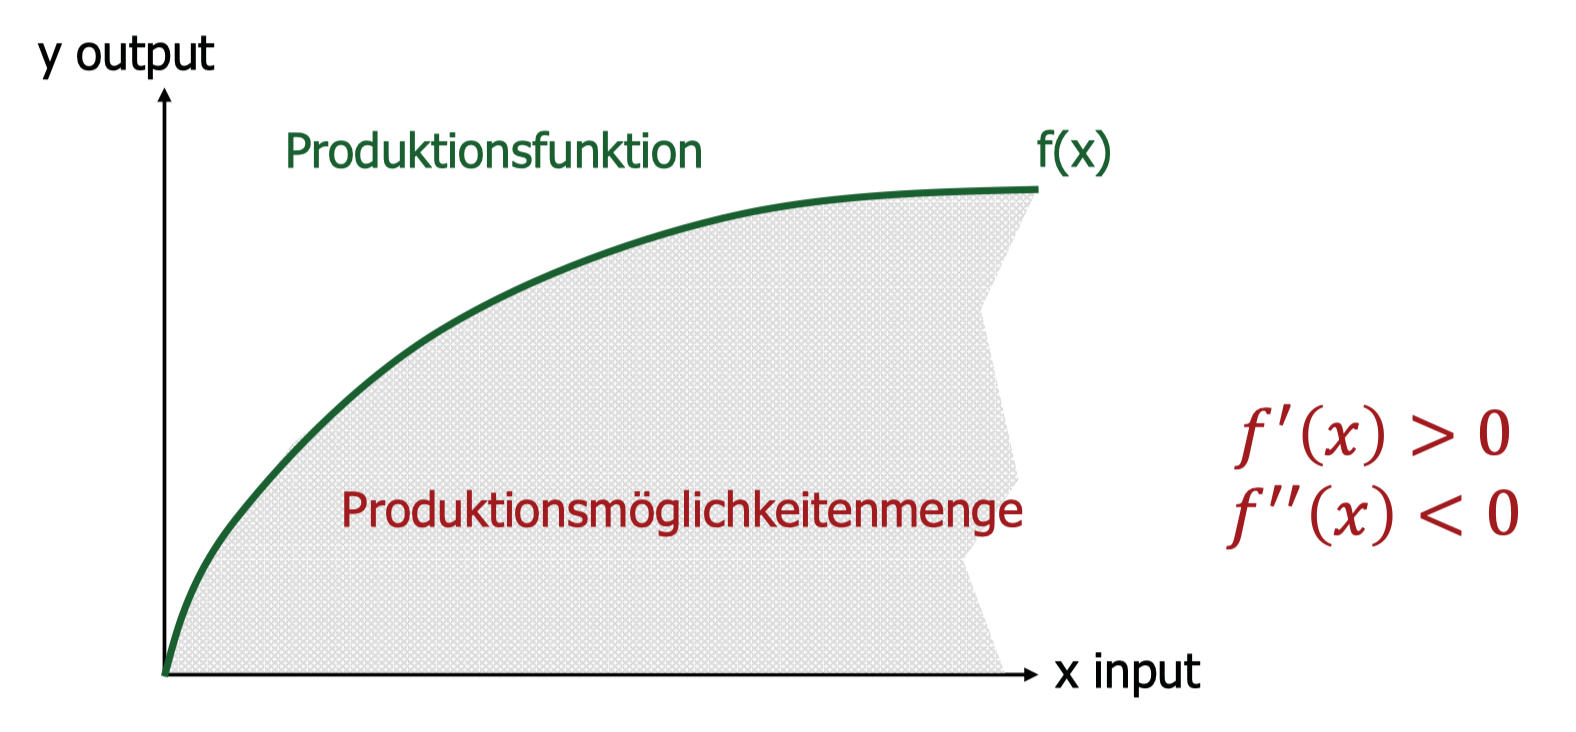
\includegraphics[scale=0.225]{img/technologiemenge}
	\end{minipage}
\end{figure} 

Eine Produktion ist \textbf{technisch effizient}, wenn ein vorgegebener Output mit geringst möglichen Inputmengen hergestellt wird. Analog ist eine Allokation technisch effizient, wenn es nicht möglich ist, die Produktionsmenge (PM) eines Gutes zu erhöhen, ohne gleichzeitig die PM eines anderen Gutes zu reduzieren.

\begin{itemize}
	\item effiziente Produktionspläne liegen auf dem Rand der Technologiemenge. Dieser Rand wird durch die Produktionsfunktion beschrieben. Diese gibt für jede Menge an Inputs die maximal mögliche Outputmenge an: $y = f(x_1, \dotsc, x_n)$
\end{itemize}

Wir nennen
\begin{itemize}
	\item eine Technologie \textbf{monoton}, wenn eine Inputerhöhung, zu keiner Outputverringerung führt ($\frac{\partial f}{\partial x_i} \geq 0$).
	\item eine Technologie \textbf{konvex}, wenn für beliebige Inputkombinationen $z$ and $x$, mit $y = f(z) = f(x)$, gilt, dass deren Mischung $\lambda z + (1-\lambda) x$ mindestens $y$ Outputeinheiten erzeugt werden, d.h. $f(\lambda z + (1-\lambda)x) \geq y$, $(0 < \lambda < 1)$.
\end{itemize}

Bei der Optimierung können zwei Fälle auftreten. Von einer Betrachtung in der kurzen Frist wird dann gesprochen, wenn mindestens ein Produktionsfaktor nicht unmittelbar angepasst werden kann, also fix ist. Hier muss lediglich die Gewinnfunktion nach dem verbleibenden Faktor maximiert werden:

$$ \max_{x_1} p f(x_1, \overline{x_2}) - w_1 x_1 - \underbrace{w_2 \overline{x_2}}_{\text{Fixkosten}} $$

Langfristig Frist können alle allerdings alle Produktionsfaktoren angepasst werden und die Optimierung ist etwas komplizierter.

\subsubsection*{Grenzprodukte der Inputfaktoren}

Das Grenzprodukt eines Inputfaktors $i$ gibt an, um wieviel der Output $y$ steigt, wenn die Einsatzmenge des Faktors $i$ geringfügig erhöht wird.
$$ MP_i = \frac{\partial f(x_1, x_2)}{\partial x_i} \geq 0 $$

\subsubsection*{Isoquanten und TRS}

Analog zu Indifferenzkurven sind Isoquanten alle technisch effizienten Inputkombinationen die zu gleichem Output führen. Die (negative) Steigung der Isoquanten ist die Technische Rate der Substitution. Sie gibt das Verhältnis an, in dem Input 2 durch Input 1 bei konstanten Output substituiert werden kann.
$$ TRS = - \frac{MP_1}{MP_2} = - \frac{\partial f(x_1, x_2)}{\partial x_1} \big/ \frac{\partial f(x_1, x_2)}{\partial x_2} $$
% todo beispiel

Achtung! Produktionsfunktionen kann man nicht positiv monoton transformieren, da sie kein rein ordinales Konzept wie die Nutzenfunktionen sind.

Außerdem ist zu beachten, dass oft es zunehmend schwieriger wird einen der Produktionsfaktor durch einen anderen bei konstantem Output zu substituieren. Dies wird als abnehmende Technische Rate der Substitution (im Absolutwert) bezeichnet.

\begin{figure*}[!htbp] \centering
	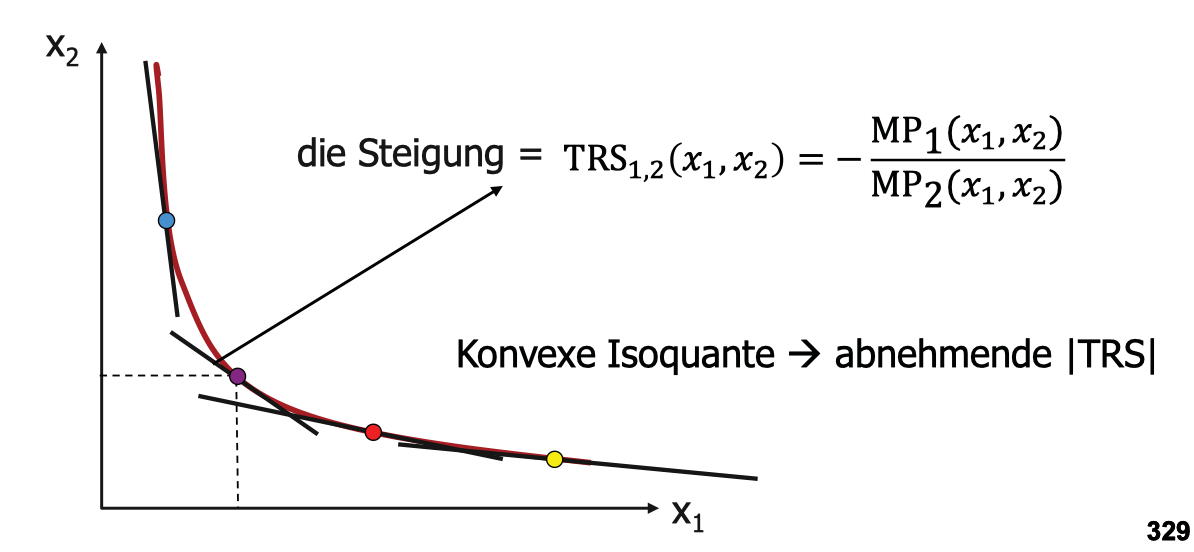
\includegraphics[scale=0.4]{img/trs}
\end{figure*}

% klassische vs neoklassische Produktionsfunktion

\subsubsection*{Skalenerträge}
Gegeben: $f(x_1, x_2)$. Wie verhält sich die Output-Menge bei Ver-t-fachung aller Inputgüter?
\begin{description}
	\item[\hspace{0.5cm}1. Fall:] $f( t \cdot x_1, t \cdot x_2) < t \cdot f(x_1, x_2)$: fallende Skalenerträge 
	\item[\hspace{0.5cm}2. Fall:] $f( t \cdot x_1, t \cdot x_2) = t \cdot f(x_1, x_2)$: kostante Skalenerträge 
	\item[\hspace{0.5cm}3. Fall:] $f( t \cdot x_1, t \cdot x_2) > t \cdot f(x_1, x_2)$: steigende Skalenerträge 	
\end{description}

\section{Gewinnmaximierung}

Es bleibt auch hier die zentrale Verhaltensannahme bestehen: alle Unternehmen maximieren ihren Gewinn. Dabei ist der Erlös eines Unternehmens das Produkt aus der verkauften Menge und dem Preis für den Output. Seien $x_1$ bzw. $x_2$ die eingesetzten Input-Mengen (zur Produktion der Output-Menge $y$) sowie $w_1, w_2$ die Faktorinputpreise von Faktor 1 und 2. Es ergibt sich das \textbf{Gewinnmaximierungsproblem}:
$$ \max \Pi(x_1, x_2) = p \cdot f(x_1, x_2) - (w_1 \cdot x_1 + w_2 \cdot x_2) $$
Dabei seien 
\begin{itemize}
	\item \textbf{Erlösfunktion}: $R(x_1, x_2) = p \cdot y = p \cdot f(x_1, x_2)$; deren Ableitung ist der Grenzerlös $MR$.
	\item \textbf{Kostenfunktion}: $C(x_1, x_2, w_1, w_2) = w_1 \cdot x_1 + w_2 \cdot x_2$; deren Ableitung sind die Grenzkosten $MC$.
\end{itemize}
Im Gewinnmaximum muss durch das Gewinnmaximierungsproblem im Allgemeinen gelten, dass 
$$ TRS = - \frac{w_1}{w_1} $$
Die Lösung dieser Gleichung ergibt die \textbf{bedingten Faktornachfragen} $x_1^*(p, w_1, w_2)$ und $x_2^*(p, w_1, w_2)$. Diese geben an, welche Inputmengen ein Unternehmen nachfragen muss, um seinen Gewinn zu maximieren. Auch die bedingten Faktornachfragen sind invariant gegenüber proportionalen Anstiegen (z.B. Verdopplung) von Faktorpreisen (obwohl die Produktionskosten reagieren).

\section{Kostenminimierung}

Setzt man die bedingten Faktornachfragen in die Kostenfunktion ein, so erhält man eine Funktion die die Minimalkosten für die Produktionsmenge $y$ angibt:
	$$ C(y) = C(w_1, w_2, y) = w_1 x_1^* + w_2 x_2^* $$
Auch lassen sich die Skalenerträge von Kostenfunktionen untersuchen:
\begin{itemize}
	\item \textbf{Konstante Skalenerträge}: $C(w, y) = y \cdot C(w, y = 1)$. 
	\item \textbf{Steigende Skalenerträge}: $C(w, y) > y \cdot C(w, y = 1)$.
	\item \textbf{Fallende Skalenerträge}: $C(w, y) < y \cdot C(w, y = 1)$
\end{itemize}

Im Allgemeinen lassen sich die Kosten in zwei Teile aufteilen:
\begin{itemize}
	\item \textbf{Fixkosten} $F$: All Kosten, die unabhängig von der Produktionsmenge $y$ entstehen. Beispiel: Miete.
	\item \textbf{Variable Kosten} $C_v(y)$: Alle Kosten, die sich mit der Produktionsmenge $y$ verändern. Beispiel: Rohstoffe.
\end{itemize}

Für die folgenden Betrachtungen benötigen wir ein paar zusätzliche Begriffe:
\begin{itemize}
	\item \textbf{Grenzkosten} $MC(y)$: die Grenzkosten sind \enquote{zusätzlichen Kosten}, die durch die Produktion \enquote{einer zusätzlichen Outputeinheit} entstehen. Formal sind die Grenzkosten also die erste Ableitung der Kostenfunktion nach $y$: $C'(y)$.
	\item \textbf{Durchschnittskosten} $AC$: die Produktionskosten, die durchschnittlich auf eine einzelne Outputeinheit bei der Produktion von insgesamt $y$ Einheiten entfallen, werden als Durchschnittskosten bzw. Stückkosten bezeichnet. Formale Definition: $AC(y) = \frac{C(y)}{y}$.
	\item Analog lassen sich die durchschnittlichen Fixkosten $AFC$ und die durchschnittlichen variable Kosten $AVC$ definieren und es gilt: $AC(y) = AFC(y) + AVC(y)$.
\end{itemize}

Es gilt: die Grenzkostenkurve ($MC$-Kurve) schneidet die Durschnittskostenkurve ($AC$-Kurve) in ihrem Minimum.